\documentclass[11pt,a4paper]{article}
\usepackage[utf8]{inputenc}
\usepackage[T1]{fontenc}
\usepackage{amsmath,amssymb,bm}
\usepackage{txfonts}
\usepackage[margin=2.4cm]{geometry}
\usepackage{graphicx}
\usepackage{booktabs,multirow}
\usepackage{caption,subcaption}
\usepackage[dvipsnames]{xcolor}
\usepackage{microtype}
\usepackage[colorlinks=true,linkcolor=MidnightBlue,citecolor=MidnightBlue,urlcolor=MidnightBlue]{hyperref}

\renewcommand{\figurename}{Figura}
\renewcommand{\tablename}{Tabla}
\renewcommand{\abstractname}{Resumen}
\renewcommand{\contentsname}{Contenido}
\renewcommand{\refname}{Referencias}
\captionsetup{font=small,labelfont=bf}
\graphicspath{{figuras/}}

\newcommand{\SoloLDos}{17}
\newcommand{\SoloLUno}{3}
\newcommand{\GanaWarmCold}{8}
\newcommand{\GanaCold}{12}
\newcommand{\GanaWarmFija}{5}
\newcommand{\GanaFija}{3}
\newcommand{\TotalCorridas}{260}
\newcommand{\FallasLUno}{41}
\newcommand{\PerdidasLUno}{11}
\newcommand{\ConvergenLUno}{58}
\newcommand{\SanidadMaxDif}{$7.7\times10^{-12}$}
\newcommand{\CompEmpates}{35}
\newcommand{\CompGanamos}{4}
\newcommand{\CompGanaEl}{1}
\newcommand{\CompTotal}{40}
\newcommand{\AlfaVar}{0.38}
\newcommand{\RazonVarDiseno}{241}
\newcommand{\NTreceK}{64}
\newcommand{\NTrecePmax}{$2.9\times10^{-3}$}
\newcommand{\NTreceKmax}{12}
\newcommand{\NTrecePfin}{$3.1\times10^{-45}$}
\newcommand{\NTreceHoras}{7.7}
\newcommand{\OrdSiempre}{9}
\newcommand{\OrdNunca}{3}
\newcommand{\OrdDepende}{8}
\newcommand{\OrdTasaAsc}{50}
\newcommand{\OrdTasaMedia}{66}
\newcommand{\OrdAscFallaEnDep}{7}
\newcommand{\RangoOchoLUno}{3/9}
\newcommand{\RangoDiecLUno}{10/20}
\newcommand{\RangoOchoLDos}{8/9}
\newcommand{\RangoDiecLDos}{18/20}
\newcommand{\NSeisTandaUno}{2}
\newcommand{\NSeisTandaDos}{8}
\newcommand{\HilosFlips}{0}
\newcommand{\MaquinaFlips}{1}
\newcommand{\MaquinaTotal}{20}
\newcommand{\TotalTodo}{478}

\makeatletter\newcommand{\tabla}[1]{\@@input #1 }\makeatother

\newcommand{\pex}{p_{\rm \acute{e}xito}}
\newcommand{\ket}[1]{|#1\rangle}

\title{\textbf{Qudit-ADAPT para Multiway Number Partitioning}\\[4pt]
\large Informe de avance}
\date{28 de septiembre de 2026}
\author{}

\begin{document}
\maketitle
\vspace{-1.5em}

\begin{abstract}
Extendemos Qudit-ADAPT al problema de partición de números en tres
subconjuntos (\emph{multiway number partitioning}, $k=3$), en el que cada número
se codifica en un qutrit y su nivel es la caja a la que se asigna. Construimos un
motor de simulación que evita toda matriz densa y entrega gradientes analíticos
al optimizador, lo validamos contra la implementación de J.~Molina
reconstruyendo sus 40 ansätze con diferencia máxima de energía
\SanidadMaxDif, y lo usamos para correr \TotalTodo{} simulaciones en BitWit
sobre instancias de $n=5$ a $10$ qutrits con solución única. El pool de orden
$\ell=2$ resuelve muchas más instancias que el de $\ell=1$, pero la tasa de éxito
cae con $n$ para ambos. La comparación entre inicializar desde el óptimo anterior
(\emph{warm start}) y desde $\bm\theta=0$ no arroja un efecto consistente con la
estadística actual. El hallazgo principal es metodológico: el resultado de una
corrida individual depende del orden, arbitrario, en que se asignan los números a
los qutrits, porque los empates en la selección de operadores se resuelven por
índice. Promediar sobre órdenes cambia la tasa de éxito medida de
\OrdTasaAsc\,\% a \OrdTasaMedia\,\% en $n=6$, y obliga a rediseñar el protocolo
antes de ampliar la estadística.
\end{abstract}

\tableofcontents

%==============================================================================
\section{Introducción}
%==============================================================================

Qudit-ADAPT es una versión para qudits de ADAPT-VQE en la que el ansatz se
construye de a un operador por vez, eligiendo en cada paso el de mayor gradiente
dentro de un pool derivado de un potencial de gauge adiabático aproximado. En el
manuscrito se aplicó a Max 3-Cut. Aquí lo extendemos a un segundo problema de
optimización ternaria: repartir $n$ números positivos en tres cajas de modo que
sus sumas queden lo más parejas posible.

El problema es natural para qutrits. Con qubits, una etiqueta de tres valores
requiere codificación \emph{one-hot} y un término de penalización que prohíba los
estados inválidos; con un qutrit por número, cada estado de la base es una
asignación válida y el nivel del qutrit \emph{es} la caja.

J.~Molina implementó una primera versión y la corrió para $n=5$ y $6$. Este
informe describe una reimplementación orientada a llegar a tamaños mayores, un
benchmark sistemático hasta $n=10$, y los resultados obtenidos hasta ahora. Los
objetivos son tres:
\begin{enumerate}
\item comparar las dos truncaciones del pool, $\ell=1$ y $\ell=2$, a lo largo de $n$;
\item poner a prueba la conjetura de que, en este problema, partir del óptimo
  anterior (\emph{warm start}) es una desventaja frente a partir de la
  superposición uniforme;
\item contar el costo en parámetros y en compuertas nativas.
\end{enumerate}

%==============================================================================
\section{Metodología}
%==============================================================================

\subsection{Formulación}

Sean $a_1,\dots,a_n$ los números y $z_j\in\{0,1,2\}$ la caja asignada al número
$j$. Seguimos la formulación de J.~Molina (\texttt{formulacion\_qubo.pdf}): con
$\Sigma_i(z)=\sum_j a_j\,\delta_{i,z_j}$ la suma de la caja $i$ y
$\mu=\tfrac13\sum_j a_j$,
\begin{equation}
  C(z)=\sum_{i=0}^{2}\big[\Sigma_i(z)-\mu\big]^2 ,
  \label{eq:costo}
\end{equation}
que vale exactamente cero en una partición perfecta. La etiqueta de cada qutrit
es el autovalor del operador dígito $\hat d=\hat J_z+\hat I$; como
$\hat J_z=\mathrm{diag}(1,0,-1)$, el nivel $m$ del qutrit lleva la etiqueta $2-m$.
Adoptamos esta convención para que las cadenas de trits se lean igual que en su
trabajo.

El Hamiltoniano de costo coincide, salvo una transformación afín, con el de
Max 3-Cut sobre el grafo completo con pesos $a_ia_j$:
\begin{equation}
  H_C=2\,H_{\rm 3\text{-}cut}^{(a_ia_j)}+\tfrac23\Big(\sum_j a_j\Big)^2 ,
\end{equation}
lo que verificamos numéricamente con residuo nulo. Dos consecuencias importan.
Como todos los pares se acoplan, el pool de una instancia de $n$ números es el
pool del grafo completo $K_n$, que es el caso más denso. Y el error relativo
$|E-E_0|/|E_0|$ no sirve aquí: en instancias balanceadas $E_0=0$ y el cociente se
indefine. Reportamos por eso energías en la escala de la ec.~\eqref{eq:costo},
donde $E$ es la desviación cuadrática media de las sumas de las cajas.

\subsection{Pool de operadores}

El pool se obtiene de los conmutadores anidados del Hamiltoniano adiabático,
truncados a orden $\ell$: con $\ell=1$ se usa $O_1$ y con $\ell=2$ se agrega $O_3$.
Sobre $K_n$, el pool de $\ell=1$ tiene exactamente $2n^2-n$ operadores (190 en
$n=10$) y el de $\ell=2$ crece como $n^{3.65}$ (18\,100 en $n=10$). Cada
operador actúa sobre a lo más cuatro qutrits.

\subsection{Motor de simulación}

El código original de la línea Max 3-Cut no escala más allá de $n\approx8$, por
dos razones evitables. Construía $H_C$ como matriz densa de $(3^n)^2$ entradas y
la diagonalizaba (52\,GB en $n=10$), y guardaba en forma densa la base propia de
cada operador del ansatz (1.4\,GB por operador en $n=8$). Ninguna de las dos
hace falta:
\begin{itemize}
\item $H_C$ es diagonal en la base computacional, así que se guarda como un
  vector de $3^n$ entradas y $E_0$ es su mínimo; el estado de referencia es el
  producto conocido $\ket{+_3}^{\otimes n}$.
\item Cada operador del pool actúa en a lo más cuatro sitios. Su bloque de
  $3^w\times3^w$ ($81\times81$ como máximo) se diagonaliza una vez, y
  $e^{-i\theta A}$ se aplica contrayendo ese bloque contra el estado. Es exacto
  incluso para los operadores cuya hermitización no factoriza como producto
  tensorial.
\item El gradiente es analítico, por el método adjunto: una pasada hacia adelante
  y una hacia atrás, con costo del orden de dos evaluaciones de la energía. Se
  entrega a BFGS junto con la función de costo (\texttt{jac=True}). Verificado
  contra diferencias finitas a $10^{-8}$.
\item La expansión simbólica del pool se hace sólo hasta el orden que $\ell$
  requiere y se guarda en disco. Los pools de $n=6$ a $14$ con $\ell=1$ se
  construyen en menos de dos segundos, y el de $n=10$ con $\ell=2$ en 3.6\,s.
\end{itemize}

\subsection{Instancias}

Cada instancia cumple tres criterios, verificados por enumeración exacta:
números \emph{distintos}; existencia de un reparto perfecto; y unicidad de ese
reparto, es decir, degeneración del fundamental exactamente igual a 6, el mínimo
posible porque cada partición aparece una vez por cada permutación de las tres
etiquetas. Los números repetidos se excluyen porque inflan la degeneración y con
ella la probabilidad de acertar por azar. Con números distintos no existe reparto
perfecto para $n<5$, por lo que el benchmark cubre $n=5,\dots,10$.

Los números se sortean en $[1,3n]$. El rango crece con $n$ porque, fijo en
$[1,15]$ como en las instancias de J.~Molina, en $n=10$ no queda ninguna
instancia de solución única. Se fijaron desde el comienzo 20 instancias por
tamaño, de forma determinista, aunque la primera tanda use sólo las 10 primeras;
así la segunda no se elige a posteriori. La tabla~\ref{tab:instancias} muestra
una por tamaño junto con su solución.

\begin{table}[h]
\centering
\caption{Una instancia de cada tamaño y su única partición perfecta. $\pex^{\rm azar}=6/3^n$
es la probabilidad de acertar midiendo la superposición uniforme.}
\label{tab:instancias}
\small\setlength{\tabcolsep}{4pt}
\begin{tabular}{rllll}
\toprule
$n$ & rango & $\pex^{\rm azar}$ & números & cajas óptimas \\
\midrule
\tabla{tabla_instancias.tex}
\bottomrule
\end{tabular}
\end{table}

\subsection{Protocolo y estrategias de inicialización}

ADAPT corre hasta que la norma del gradiente del pool cae bajo
$\epsilon=10^{-3}$ (en la escala de la ec.~\ref{eq:costo}) o hasta 150 parámetros.
El optimizador interno es BFGS con \texttt{gtol}$\,=10^{-10}$. Se comparan tres
estrategias:
\begin{description}
\item[warm start.] El ADAPT estándar: cada optimización parte de
  $(\bm\theta^*_{k-1},0)$, el óptimo anterior más el parámetro nuevo en cero.
\item[(i) secuencia fija desde $\bm\theta=0$.] Se toma la secuencia de operadores
  que eligió la corrida warm y, para cada tamaño $k$, se reoptimiza ese mismo
  circuito partiendo de cero. Aísla el efecto de la inicialización sobre un
  circuito dado; es el experimento de las Figs.~5--6 del manuscrito.
\item[(ii) ADAPT desde $\bm\theta=0$.] En cada paso se reoptimizan todos los
  parámetros partiendo de cero, es decir, desde la superposición uniforme. Como el
  estado optimizado cambia, el barrido siguiente elige otros operadores: es otro
  algoritmo, y es la variante que pone a prueba la conjetura.
\end{description}

\subsection{Métricas}

La métrica principal es $\pex$, el peso del estado final sobre el subespacio de
las soluciones óptimas: la probabilidad de que una medición entregue la
partición correcta. Consideramos una instancia \emph{resuelta} si
$\pex\geq0.1$; con esa probabilidad, 50 mediciones bastan para ver la solución
con más de 99\,\% de certeza, y verificar cuál de ellas es óptima es trivial
clásicamente. Un criterio más estricto, pedir que la cadena más probable sea la
correcta, cuenta como fallas estados con la mitad de su peso sobre la solución, y
lo descartamos.

Se registran además, en cada iteración, la energía, la norma del gradiente,
$\pex$, los parámetros, los empates en la selección y los tiempos; el número de
parámetros, las compuertas nativas según el Algoritmo~1 de Ringbauer
\emph{et~al.} y el commit exacto del código que produjo cada resultado.

\subsection{Validación y ejecución}

El código de J.~Molina no corre desde un clon del repositorio porque depende de
un módulo que no está publicado, pero sus resultados guardan los operadores y
parámetros finales de cada corrida. Reconstruimos sus 40 ansätze en nuestro motor
y comparamos la energía del estado resultante con la suya.

Todas las corridas del benchmark se hicieron en BitWit (AMD Threadripper 7980X,
64 núcleos, 125\,GB), en paralelo, con varios procesos de pocos hilos de BLAS cada uno, a partir de árboles exportados de commits fijos del
repositorio.

%==============================================================================
\section{Resultados}
%==============================================================================

\subsection{Validación contra la implementación de J. Molina}

Los 40 ansätze reconstruidos dan su energía con diferencia máxima \SanidadMaxDif,
y la probabilidad de la cadena más probable coincide en los 40. Las dos
implementaciones concuerdan en el estado de referencia, la hermitización del
pool, las convenciones de signo y de orden, y el Hamiltoniano.

Corriendo además nuestro ADAPT sobre sus 40 instancias con sus mismos ajustes
($\epsilon=10^{-3}$, tope de 30), $\pex$ coincide dentro de 0.05 en \CompEmpates{}
de \CompTotal{} casos; en \CompGanamos{} el nuestro llega más alto y en
\CompGanaEl{} el suyo. Las diferencias vienen de que su pool contiene $n$
operadores de un sitio más: sus proyectores son cuadráticos en $\hat d$ y la
expansión simbólica produce más monomios distintos.

\subsection{Fase 1: \texorpdfstring{$\ell=1$}{l=1} contra \texorpdfstring{$\ell=2$}{l=2}}

La tabla~\ref{tab:fase1} y la figura~\ref{fig:exito} resumen las 120 corridas con
warm start. El pool de $\ell=2$ resuelve muchas más instancias: sobre la misma
instancia, $\ell=2$ acierta y $\ell=1$ no en \SoloLDos{} casos, y lo contrario
ocurre en \SoloLUno. Para ambos pools la tasa de éxito cae con $n$, y en $n=10$
casi ninguna instancia se resuelve.

\begin{table}[h]
\centering
\caption{Fase 1, warm start, 10 instancias por tamaño. ``Conv.'' cuenta las
corridas que terminaron por el criterio de gradiente y no por el tope de 150
parámetros; ``nativas'' y ``MS'' son medianas del total de compuertas nativas y de
compuertas Mølmer--Sørensen.}
\label{tab:fase1}
\small
\begin{tabular}{rrcccrccr}
\toprule
$n$ & $\ell$ & resueltas & $\pex$ mediana & $k$ med. & conv. & nativas & MS & tiempo \\
\midrule
\tabla{tabla_fase1.tex}
\bottomrule
\end{tabular}
\end{table}

\begin{figure}[h]
\centering
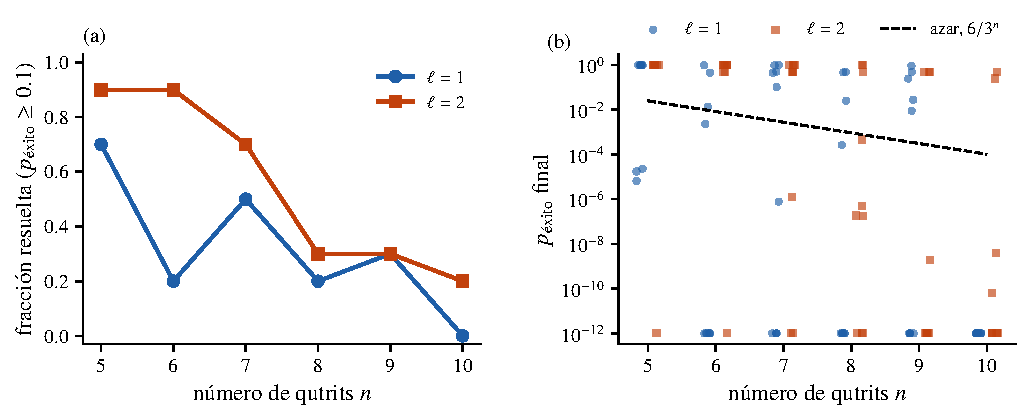
\includegraphics[width=\textwidth]{exito_vs_n}
\caption{(a) Fracción de instancias resueltas ($\pex\geq0.1$) en función de $n$.
(b) $\pex$ final de cada instancia; la línea discontinua es el azar, $6/3^n$. Las
probabilidades menores que $10^{-12}$ se grafican sobre el piso.}
\label{fig:exito}
\end{figure}

Dos salvedades. Con $\ell=1$, \ConvergenLUno{} de las 60 corridas convergieron
por el criterio de gradiente: sus fallas son mínimos locales genuinos, no falta
de presupuesto. Con $\ell=2$, en cambio, muchas corridas de $n\geq7$ llegaron al
tope de 150 parámetros (tabla~\ref{tab:fase1}), así que sus resultados ahí son
cotas inferiores.

\subsection{Respuestas perdidas}

En \PerdidasLUno{} de las \FallasLUno{} corridas con $\ell=1$ que no resuelven la
instancia, $\pex$ llegó a mitad de camino a más de diez veces el azar antes de
caer. La figura~\ref{fig:trazas} muestra dos casos. En ambos el warm start sube
$\pex$ por encima del 10\,\% y después la lleva a menos de $10^{-12}$ mientras la
energía sigue bajando. Minimizar $\langle H_C\rangle$ no exige concentrarse en la
solución: basta con repartir el peso sobre configuraciones cercanas, y el fondo
del espectro de este problema es denso.

\begin{figure}[h]
\centering
\begin{subfigure}{0.49\textwidth}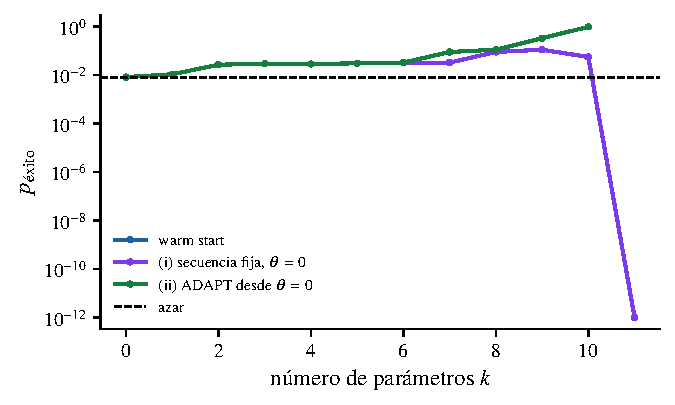
\includegraphics[width=\textwidth]{trazas_n6_i03}
\caption{$n=6$, instancia 3.}\end{subfigure}\hfill
\begin{subfigure}{0.49\textwidth}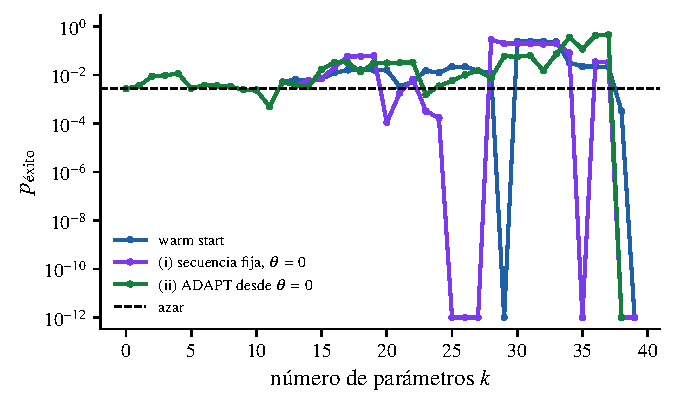
\includegraphics[width=\textwidth]{trazas_n7_i04}
\caption{$n=7$, instancia 4.}\end{subfigure}
\caption{$\pex$ en función del número de parámetros para las tres estrategias.
En (a), el warm start alcanza $\pex=0.11$ y la pierde, la misma secuencia
reoptimizada desde cero también falla, y ADAPT desde cero acierta con
$\pex=0.97$. En (b) ninguna estrategia la recupera.}
\label{fig:trazas}
\end{figure}

\subsection{Fase 2: warm start contra \texorpdfstring{$\bm\theta=0$}{theta=0}}

La tabla~\ref{tab:fase2} y la figura~\ref{fig:pareado} comparan las tres
estrategias con $\ell=1$ sobre las mismas instancias. Contamos que una estrategia
``gana'' cuando su $\pex$ es más del doble de la otra y mayor que $10^{-6}$.

\begin{table}[h]
\centering
\caption{Fase 2 con $\ell=1$. Las tres primeras columnas son instancias
resueltas de 10; las dos últimas, comparaciones instancia a instancia en la forma
``gana warm / gana la otra / empate''.}
\label{tab:fase2}
\small
\begin{tabular}{rccccc}
\toprule
 & \multicolumn{3}{c}{resueltas} & \multicolumn{2}{c}{contra warm} \\
\cmidrule(lr){2-4}\cmidrule(lr){5-6}
$n$ & warm & (ii) & (i) & (ii) ADAPT desde 0 & (i) secuencia fija \\
\midrule
\tabla{tabla_fase2.tex}
\bottomrule
\end{tabular}
\end{table}

\begin{figure}[h]
\centering
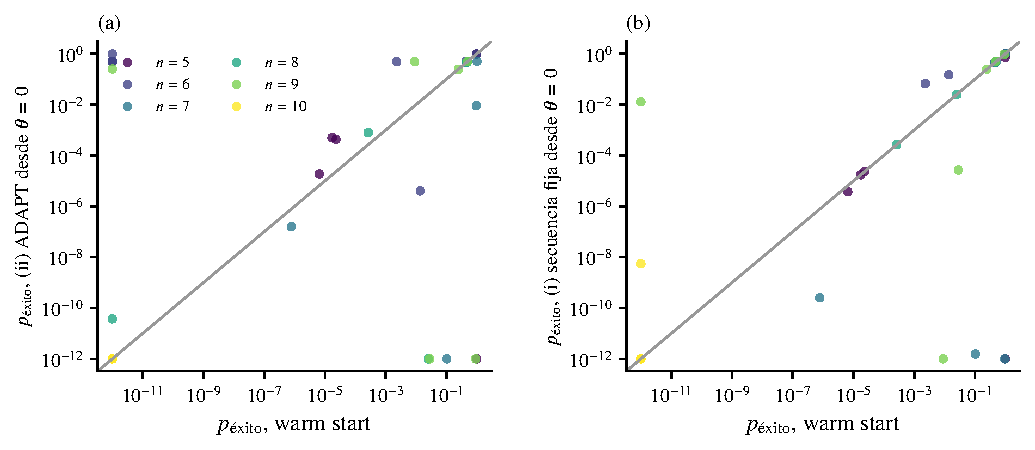
\includegraphics[width=\textwidth]{pareado_warm_cold}
\caption{$\pex$ de cada instancia con warm start contra (a) ADAPT desde
$\bm\theta=0$ y (b) la secuencia fija reoptimizada desde cero. Sobre la diagonal,
gana la estrategia del eje vertical.}
\label{fig:pareado}
\end{figure}

ADAPT desde $\bm\theta=0$ gana en \GanaCold{} instancias y el warm start en
\GanaWarmCold, pero el signo depende de $n$: en $n=6$ gana (ii) por seis a uno y
en $n=7$ gana warm por tres a cero. Con la secuencia fija, el warm start es igual
o mejor (\GanaWarmFija{} a \GanaFija), lo que es coherente con el argumento de
\emph{burrowing}: sobre un circuito dado, partir del óptimo anterior garantiza un
descenso monótono.

\subsection{¿Importa el rango de los números?}

Nuestro motor resuelve las cuatro instancias sin repetidos de $n=6$ de J.~Molina,
pero sólo 2 de nuestras 10. Como sus números llegan hasta 8 y los nuestros hasta
18, probamos si la magnitud explica la diferencia. Con $n=6$, números distintos y
solución única existen exactamente 9 instancias en $[1,8]$; las corrimos todas,
junto con las 10 instancias restantes de la segunda tanda en $[1,18]$
(figura~\ref{fig:rango}).

\begin{figure}[h]
\centering
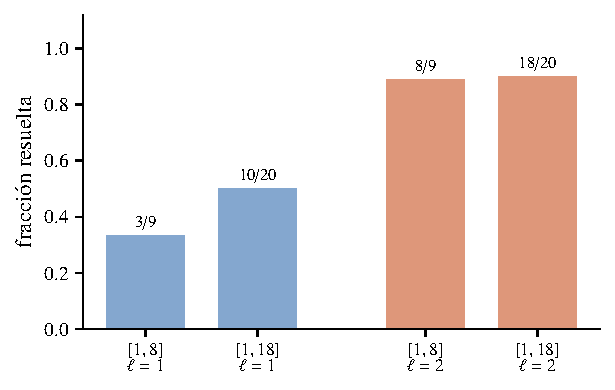
\includegraphics[width=0.52\textwidth]{rango}
\caption{Fracción resuelta en $n=6$ según el rango de los números.}
\label{fig:rango}
\end{figure}

El rango no explica nada: con $\ell=1$ se resuelven \RangoOchoLUno{} en $[1,8]$ y
\RangoDiecLUno{} en $[1,18]$, y con $\ell=2$, \RangoOchoLDos{} y \RangoDiecLDos.
Además la segunda tanda de $[1,18]$ resolvió \NSeisTandaDos{} de 10, contra
\NSeisTandaUno{} de la primera: el resultado de la fase 1 en $n=6$ era una muestra
desfavorable, no una propiedad de las instancias.

\subsection{Sensibilidad al orden de los números y a la máquina}

La diferencia con J.~Molina resultó venir de otro lado. Nuestro benchmark ordena
los números de menor a mayor antes de asignarlos a los qutrits; él no. Con los
mismos números en su orden y $\ell=1$, las dos instancias de $[1,8]$ que coinciden con las
suyas se resuelven con $\pex=0.49$ y $0.97$; ordenadas, con $\pex=0$.

Permutar qué número va en qué qutrit no cambia el problema, pero sí puede
cambiar la trayectoria de ADAPT. Cuando varios operadores empatan en el gradiente,
\texttt{argmax} toma el de menor índice, y el índice depende del etiquetado; un
solo empate basta para que dos trayectorias diverjan. Para cuantificarlo corrimos
las 20 instancias de $n=6$ bajo 10 órdenes cada una (figura~\ref{fig:ordenes}).
\OrdSiempre{} se resuelven en cualquier orden, \OrdNunca{} en ninguno y
\OrdDepende{} dependen del orden. Con el orden ascendente se resuelve el
\OrdTasaAsc\,\%; promediando sobre órdenes, el \OrdTasaMedia\,\%.

\begin{figure}[h]
\centering
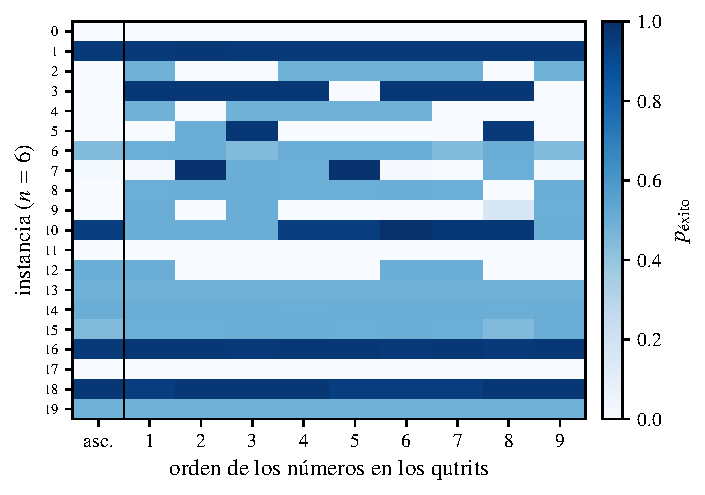
\includegraphics[width=0.6\textwidth]{ordenes}
\caption{$\pex$ de las 20 instancias de $n=6$ ($\ell=1$, warm start) bajo 10
órdenes de sus números. La primera columna es el orden ascendente del benchmark.}
\label{fig:ordenes}
\end{figure}

El orden ascendente parece además sistemáticamente desfavorable: de las
\OrdDepende{} instancias que dependen del orden, falla en \OrdAscFallaEnDep. Una
hipótesis, todavía sin probar, es que al desempatar por índice menor con los
números en orden creciente se favorecen operadores sobre los números más chicos,
que son los que menos pesan en el balance.

El mismo fenómeno aparece con el hardware. Repetimos en una laptop las 20
corridas de $n=5$ y $6$ con $\ell=1$: con uno o dos hilos de BLAS el veredicto no
cambia en ningún caso (\HilosFlips/\MaquinaTotal), pero entre la laptop y BitWit
cambia en \MaquinaFlips{} de \MaquinaTotal. Distintos procesadores y builds de
BLAS redondean distinto, y en un casi-empate esa diferencia de $10^{-16}$ basta
para bifurcar la trayectoria. Todas las corridas del benchmark son de BitWit y
son consistentes entre sí, pero una corrida individual no debe tomarse como
propiedad robusta de su instancia.

\subsection{Varianza del gradiente}

En un barrido anterior medimos la varianza del gradiente en puntos de parámetros
aleatorios contra el número de qutrits, de $n=6$ a $14$, con ansätze de $k=5$, 10
y 20 operadores sorteados del pool de $\ell=1$ y $H_C$ normalizado por su rango
espectral (figura~\ref{fig:varianza}). Un ajuste exponencial da
${\rm Var}\propto e^{-\alpha n}$ con $\alpha=\AlfaVar$, contra $\ln3\approx1.10$ de un
ansatz que se acerque a un 2-diseño; en $n=14$ la varianza medida es
\RazonVarDiseno{} veces mayor que la de esa referencia, y apenas cambia con la
profundidad.

\begin{figure}[h]
\centering
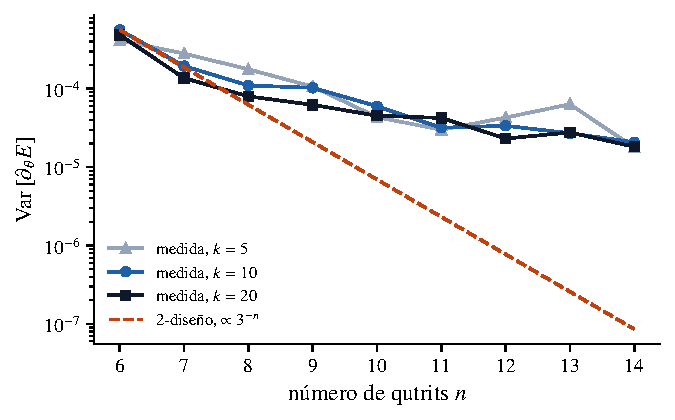
\includegraphics[width=0.55\textwidth]{varianza}
\caption{Varianza del gradiente en puntos aleatorios contra $n$, para tres
profundidades, y la referencia de un 2-diseño anclada en $n=6$.}
\label{fig:varianza}
\end{figure}

\subsection{Una instancia de \texorpdfstring{$n=13$}{n=13}}

Una corrida exploratoria con $n=13$ y $\ell=1$ convergió por gradiente en
\NTreceK{} parámetros tras \NTreceHoras\,h. La probabilidad de medir la solución
alcanzó su máximo, \NTrecePmax, en $k=\NTreceKmax$, y terminó en \NTrecePfin:
menos que el azar. Es el mismo fenómeno de la sección de respuestas perdidas,
llevado al extremo.

\subsection{Costo computacional}

Con $\ell=1$ casi todo el tiempo se va en BFGS; con $\ell=2$, entre un cuarto y casi la
mitad se va en el barrido de gradiente del pool (figura~\ref{fig:tiempos}). En
$n=10$ una corrida con $\ell=2$ toma del orden de horas. El costo por evaluación
de la energía crece entre $n=8$ y $9$ bastante más que el tamaño del estado, lo
que atribuimos a contención de memoria entre los procesos concurrentes y a copias
evitables del estado en la contracción de bloques; queda por medirlo aislado.

\begin{figure}[h]
\centering
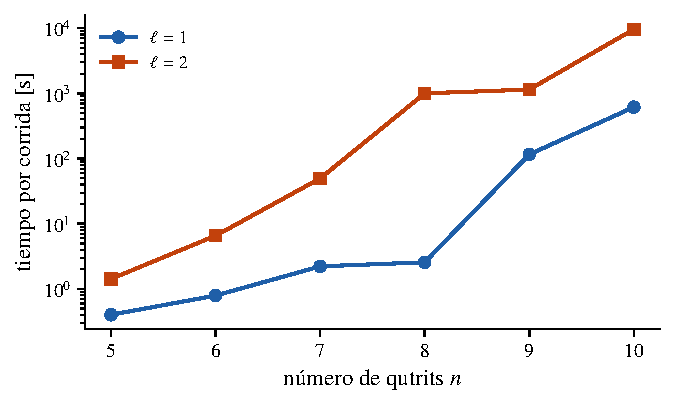
\includegraphics[width=0.55\textwidth]{tiempos}
\caption{Tiempo mediano por corrida en BitWit, con warm start.}
\label{fig:tiempos}
\end{figure}

%==============================================================================
\section{Análisis}
%==============================================================================

\paragraph{El pool importa más que la inicialización.}
Pasar de $\ell=1$ a $\ell=2$ es, con diferencia, lo que más aumenta la tasa de
éxito. El efecto de la estrategia de inicialización es, en comparación, pequeño y
de signo variable. Esto es consistente con la imagen de que el cuello está en la
expresividad del pool: $\ell=1$ contiene sólo operadores de uno y dos sitios.

\paragraph{Energía y solución se desacoplan.}
Las respuestas perdidas y la corrida de $n=13$ muestran que bajar la energía no
equivale a acercarse a la solución. El error de energía, en particular el error
relativo, es una métrica engañosa para este problema; la cifra relevante es
$\pex$.

\paragraph{La conjetura sobre el warm start sigue abierta.}
Con 10 instancias por tamaño no hay un efecto consistente. Hay, sin embargo, una
distinción que vale la pena mantener: sobre un circuito fijo el warm start no es
peor que partir de cero, así que si la conjetura resulta cierta, el mecanismo
tendría que estar en la \emph{selección} de operadores y no en la inicialización.
Una observación de avances anteriores de este trabajo, un ejemplo en que la
diferencia parecía nítida, resultó depender de la máquina en que se corrió y se
descartó.

\paragraph{El protocolo tiene que promediar sobre órdenes.}
Éste es el resultado que más condiciona lo que sigue. Si \OrdDepende{} de 20
instancias cambian de veredicto según un orden arbitrario, una sola corrida por
instancia mide tanto el orden como el algoritmo, y comparar dos estrategias sobre
un orden fijo puede reflejar cuál de ellas tuvo un empate a favor. La tasa de éxito
debe estimarse promediando sobre varios órdenes, o sobre un desempate aleatorio
con semilla, y eso vale también para reevaluar la fase 2.

\paragraph{Barren plateaus.}
La varianza del gradiente cae con $n$ mucho más lento que la de un 2-diseño y no
depende de la profundidad, lo que va en la dirección de lo que el manuscrito
afirma. Con nueve puntos entre $n=6$ y $14$, sin embargo, no se distingue un
decaimiento exponencial lento de uno polinomial: sobre ese rango las dos curvas
casi coinciden.

%==============================================================================
\section{Limitaciones y próximos pasos}
%==============================================================================

\begin{itemize}
\item \textbf{Promediar sobre órdenes.} Rehacer las fases 1 y 2 con varios
  órdenes por instancia, o con desempate aleatorio, antes de ampliar a 20
  instancias por tamaño. Probar la hipótesis de que el orden ascendente es
  desfavorable.
\item \textbf{Presupuesto de $\ell=2$.} Subir el tope de parámetros para $n\geq7$,
  donde muchas corridas no convergieron.
\item \textbf{Rendimiento.} Medir aislado el costo por evaluación, eliminar las
  copias del estado en la contracción de bloques y ajustar el número de procesos
  concurrentes al ancho de banda de memoria.
\item \textbf{Comparación con otros algoritmos.} Queda para el final, según lo
  acordado.
\item \textbf{Código de J.~Molina.} Su implementación depende de un módulo que no
  está en el repositorio; nuestro motor la reemplaza y está validado contra sus
  resultados.
\end{itemize}

\end{document}
